\section{Contour Tracing}

Contour tracing also known as boundary tracing or border following is a method of locating images in a binary image by tracing their perimeter. It does so by generating a list of coordinates that comprise the outline of a connected-component of 1-pixels. 

The specific algorithm utilized in this system works was designed by Satoshi Suzuki in 1985 \cite{satoshi_findContours}. The algorithm works by identifying that a pixel is the edge of an object, determining if the border belongs to a hole or is the outer border of an object and labelling it accordingly. An important notation when considering this algorithm is that of 4- (8-) connectedness of a 1-pixel. A 4-connected pixel is a neighbour to every one of the pixels that touches it edges and an 8-connected pixel is a neighbour to every pixel that touches it edges and corners. Connectedness is used to determine if a pixel is part of a connected-component. Figure \ref{fig:connectedness} illustrates what these connections look like and Figure \ref{fig:connection_examples} illustrates some examples of 1-pixel connected-components and how they're connected.

\begin{figure}[H]
    \centering
    \centering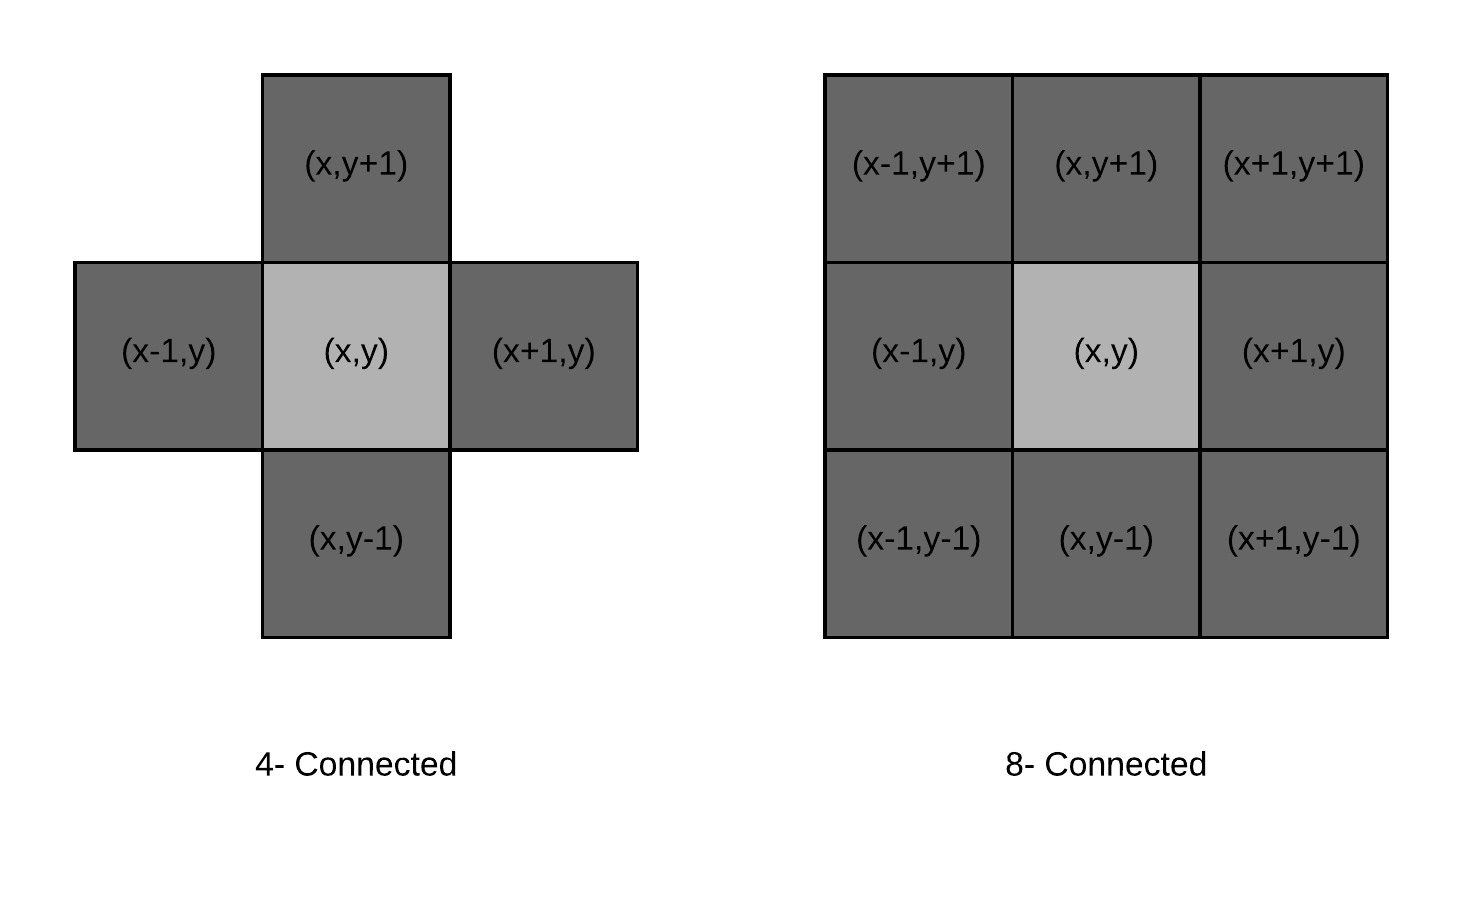
\includegraphics[width = 0.8\textwidth]{litreview/contours/connectedness.png}
    \caption{4- (8-) Connectedness of a pixel (x,y)}
    \label{fig:connectedness}
  \end{figure}

  \begin{figure}[H]
    \centering
    \centering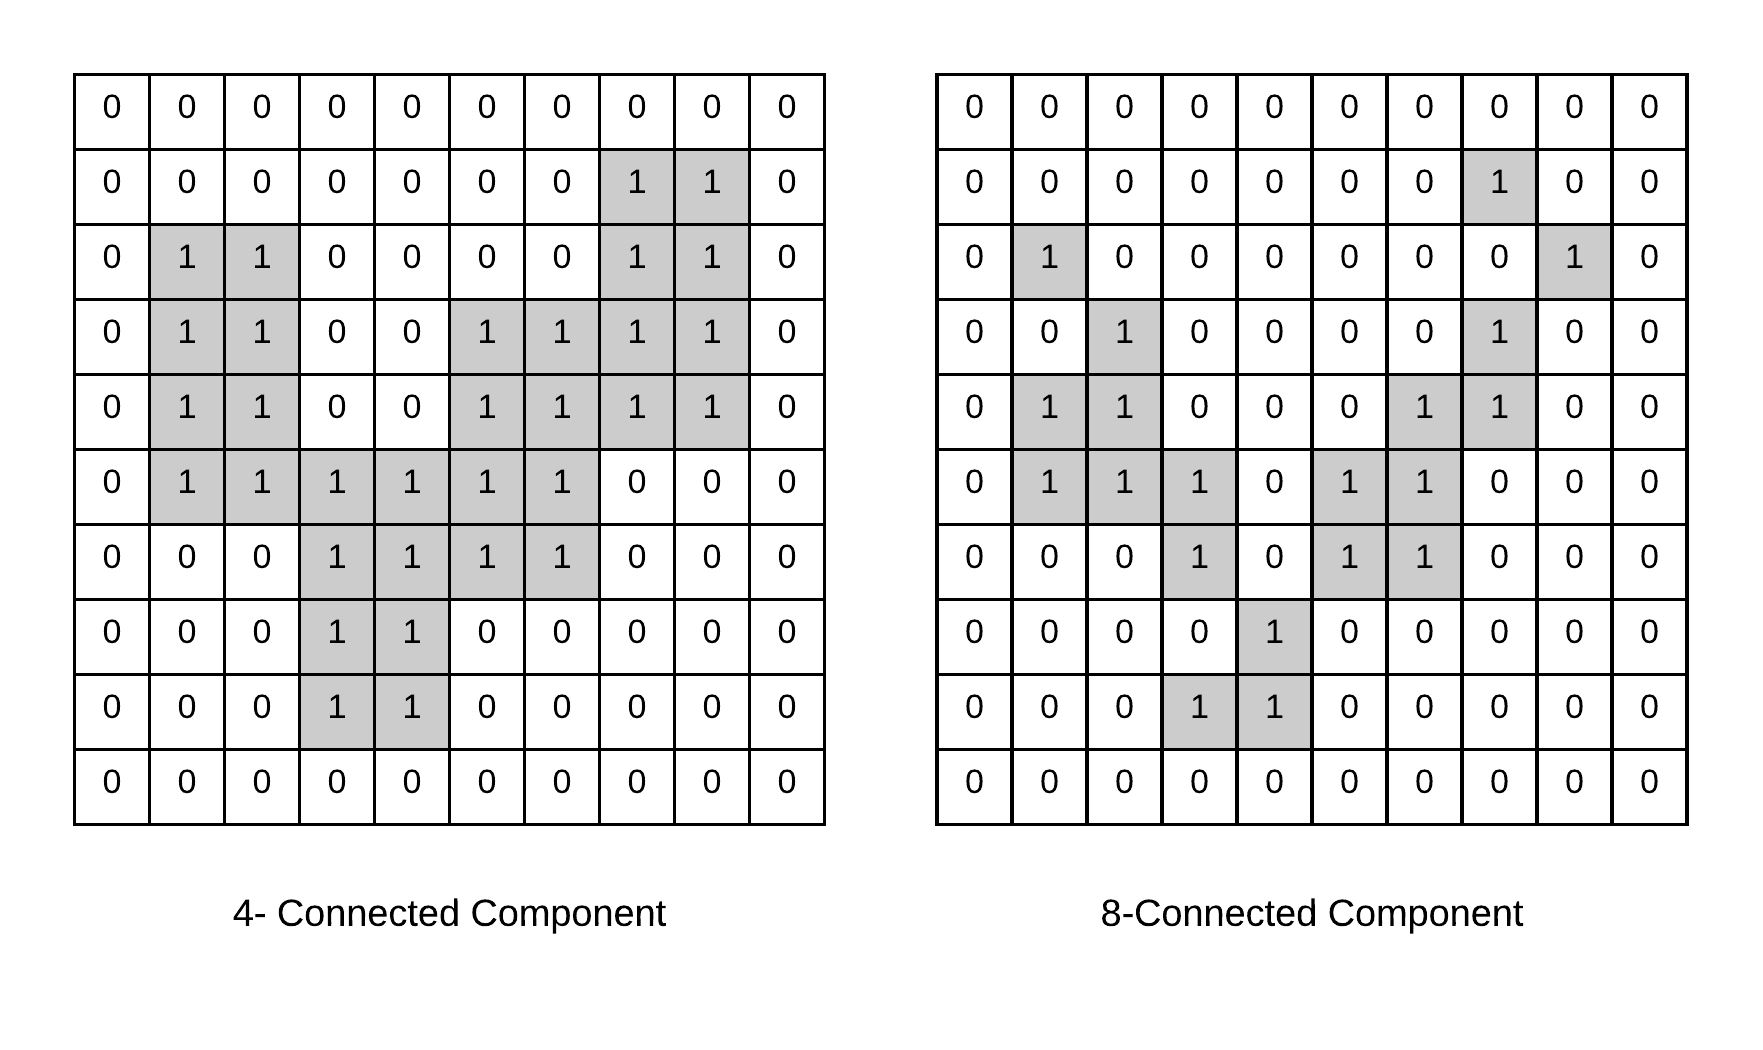
\includegraphics[width = 0.8\textwidth]{litreview/contours/connection_examples}
    \caption{Examples of different types of connected components.}
    \label{fig:connection_examples}
  \end{figure}
  

When the algorithm is performed the cells of the image are scanned in a raster fashion (left to right, top to bottom) and when a 1-pixel is encountered the algorithm interrupts and determines the type of border the pixel is that it ran into to. There are two types of border a hole border and an outer border. Figure \ref{fig:borders} illustrates these two types of borders. Satoshi defines a border point to be one that has a 0-pixel in its 4- (8-) neighborhood. An outer border is one surrounded by 0-pixel connected component and a hole border is one that surrounds a 0-pixel component. If a border is has thickness of only one pixel and is satisfies both being an outer border and hole border it's regarded as an outer border. The high-level outline of the algorithm is specified in Algorithm \ref{algorithm:satoshi} though the source material \cite{satoshi_findContours} should be consulted for a more comprehensive description.

\begin{figure}[H]
    \centering
    \centering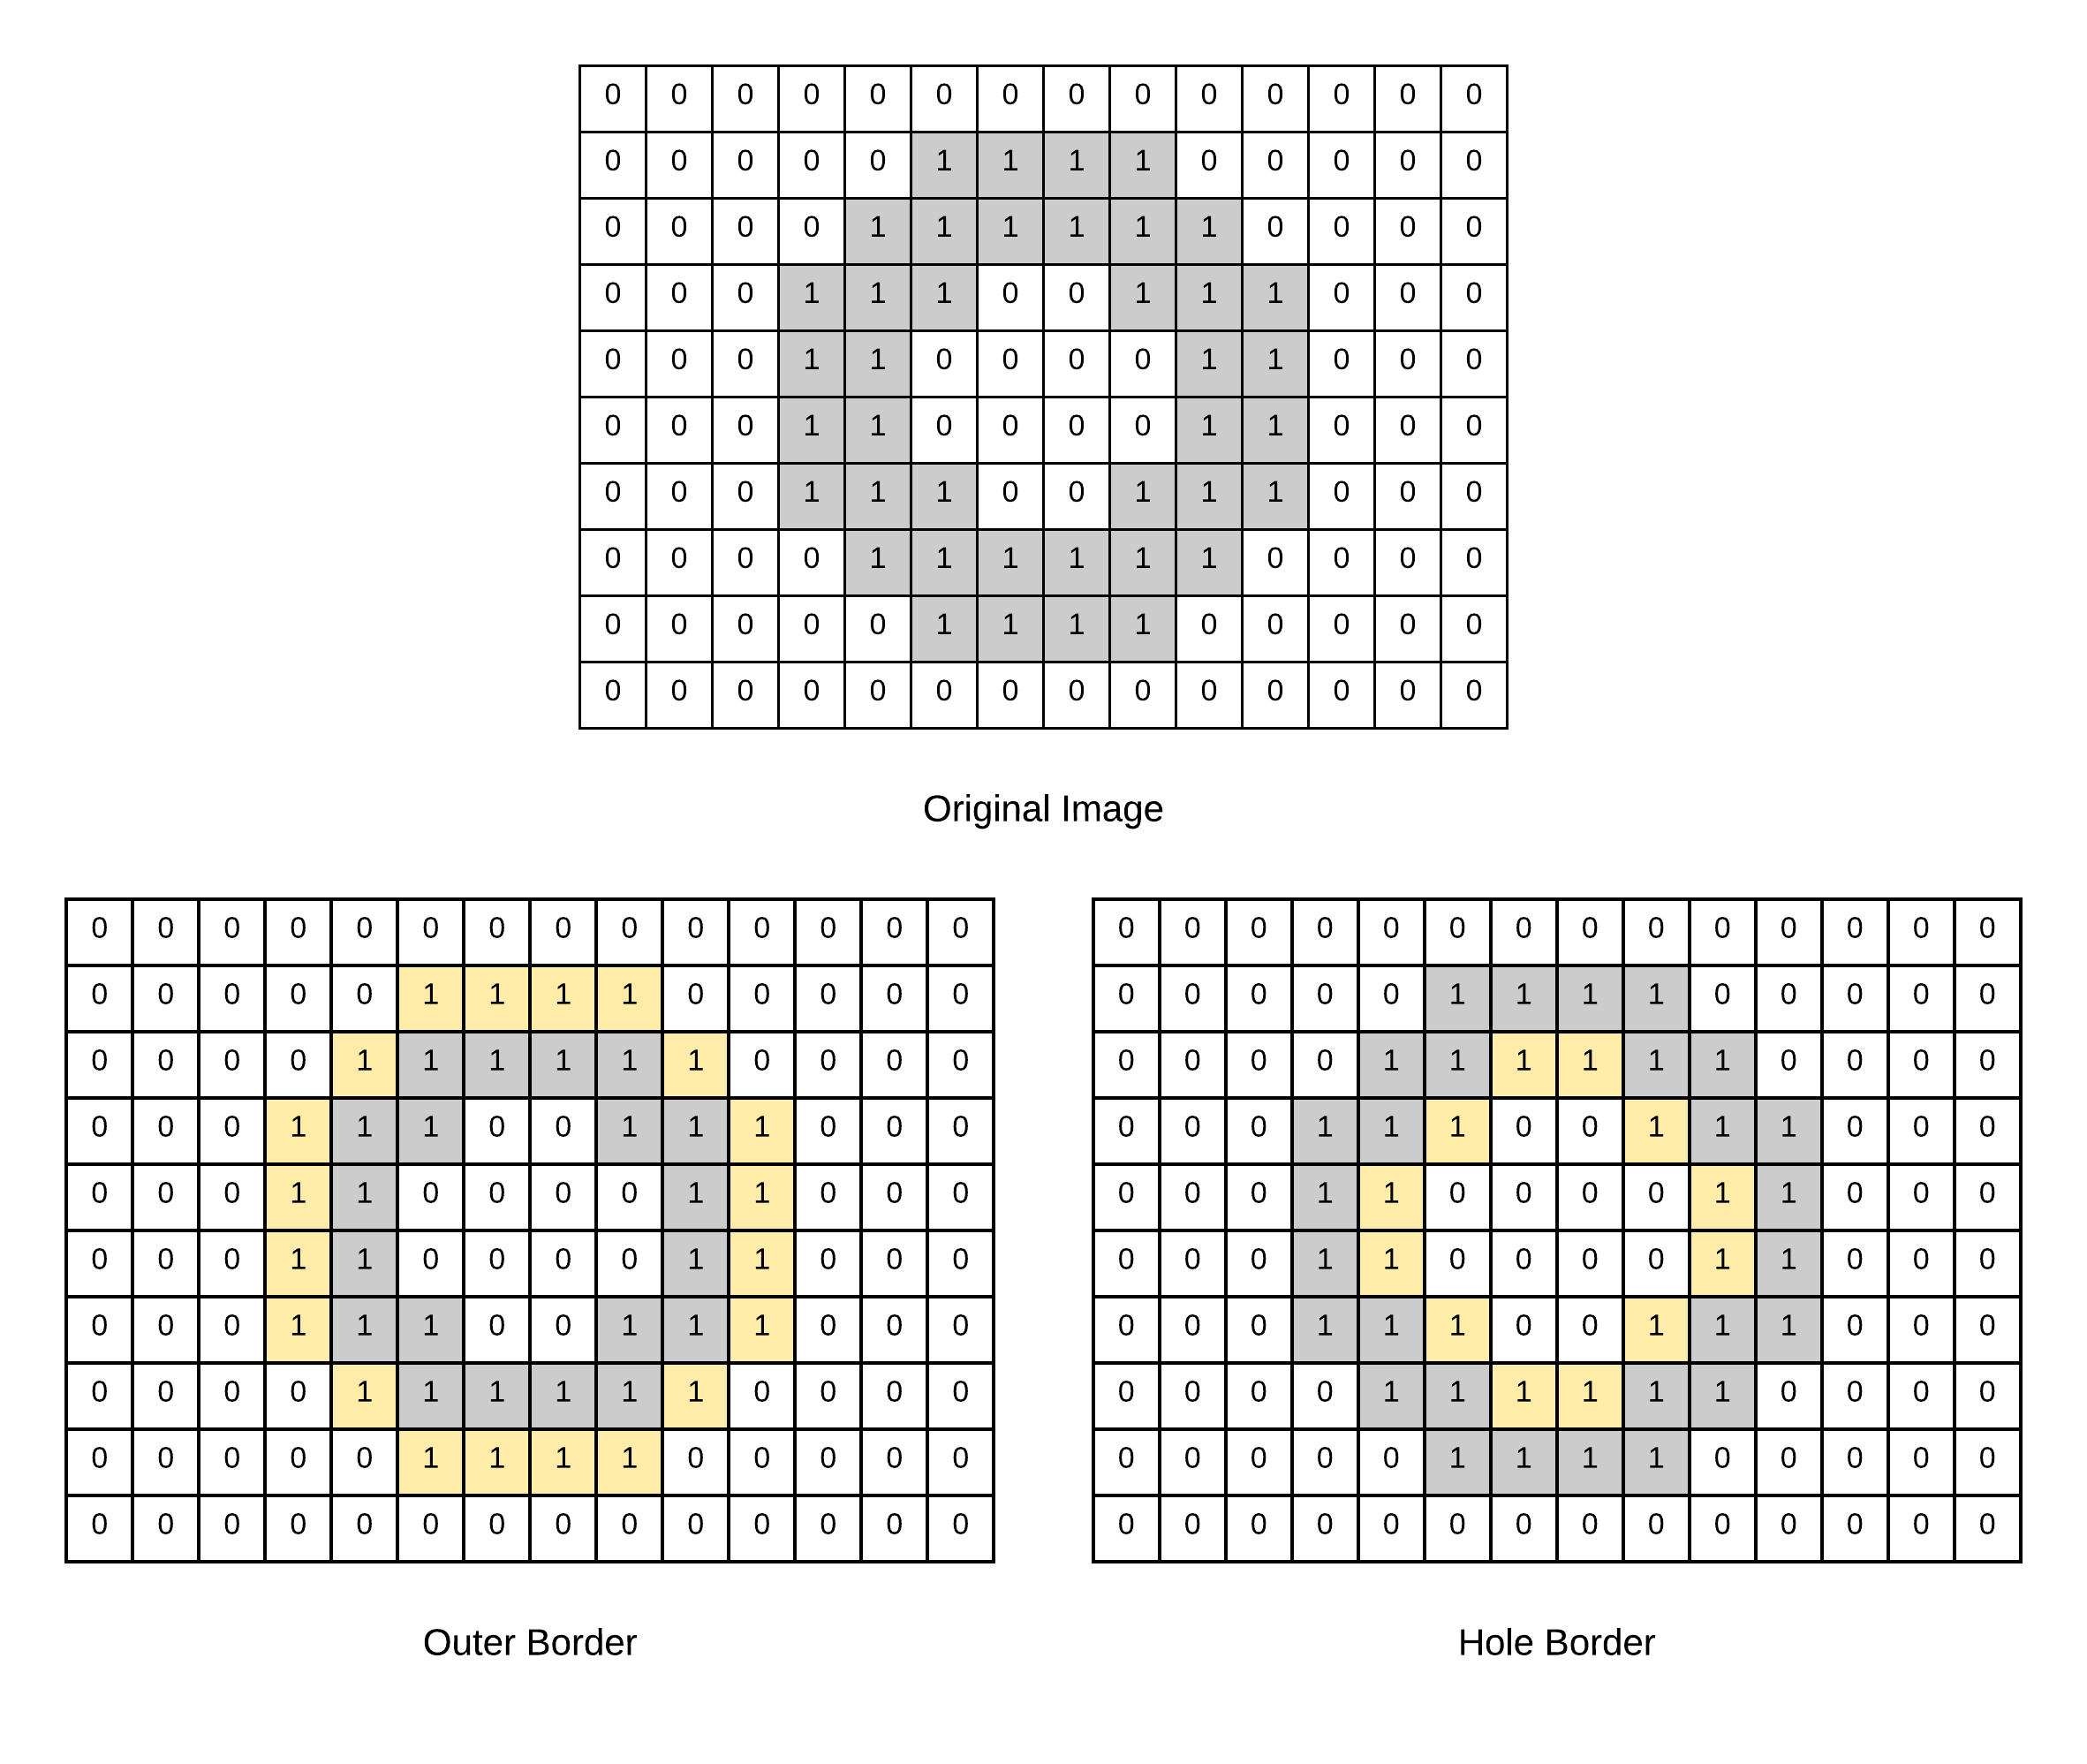
\includegraphics[width = 0.8\textwidth]{litreview/contours/borders}
    \caption{Comparison of a hole border and outer border.}
    \label{fig:borders}
  \end{figure}


\begin{algorithm}
\SetAlgoLined
\KwInput{Binary image, F, size I x J} 
\KwOutput{Coordinates of all object borders in F}
Initialize LNBM = 1 which tracks most recently labelled border.\;
Initialize counter NBD = 0 which tracks the number of borders created.\;
\While{imageScanner $\neq$ F[I,J]}{
    \uIf{F[i,j] = 1 and F[i,j-1] = 0}{
        F[i,j] is the starting point of an outer border\;
        follow border until return to starting point labelling all points with a unique ID\;
    }\uElseIf{F[i,j] $\geq$ 1 and F[i,j+1] = 0}{
        F[i,j] is the starting point of a hole border\;
        follow border until return to starting point labelling all points with a unique ID\;
    }
}
\caption{Satoshi Suzuki's algorithm for border tracing \cite{satoshi_findContours}.}
\label{algorithm:satoshi}
\end{algorithm}


  

